% Drawing 148/01-6 -- folder 148, batch 01, archive page 19 (PDF page 20).
% Transcription: en haut, une suite de croquis de sphères : à gauche une sphère à équateur avec quatre flèches ; au centre une sphère dont l'équateur porte les points $a, b$ et, au-dessus, $c, d$, d'où partent quatre flèches : vers le haut, marquée $\rho$, deux sphères et un tétraèdre ; vers la gauche, marquée $\sigma$, une sphère méridienne et deux sphères accolées, avec la lettre $\ell$ au-dessous ; vers la droite, deux sphères ; vers le bas, deux sphères et un tétraèdre
% Kind: sequence of sphere sketches with arrows. Method 2 (schematic redraw from the facsimile). Status: partial.
% Notes: Left: a sphere with equator and four arrows (up, down, left, right). Centre: a sphere whose equator carries a, b and above it c, d; four arrows: up (rho) to two spheres with meridians and a tetrahedron, left (sigma) to a sphere with a meridian and two spheres side by side, with l below; right to two spheres; down to two spheres and a tetrahedron. The dotted / solid strokes on the small spheres are schematised (equator and meridians), their marked points mostly left out.
% Coordinates: 1 unit = 1 mm = 1/100 of the crop width (bbox in page fractions: [0.1, 0.07, 0.97, 0.32]).
% Redrawn by Claude (claude-opus-5-5), issue #73, 2026-11-07; not checked by a human; not compiled (no TeX in the session).
% Rights: reproduces part of the work -- behind RENDER_TRANSCRIPTS, never published by itself.
\documentclass[tikz,border=3pt]{standalone}
\usepackage{amsmath,amssymb}
\usetikzlibrary{patterns,arrows.meta}
\tikzset{pencil/.style={black!45}, struck/.style={black!35}, mark/.style={circle,draw,inner sep=1.3pt}, pt/.style={circle,fill,inner sep=0.9pt}, opt/.style={circle,draw,fill=white,inner sep=1.1pt}}
\begin{document}
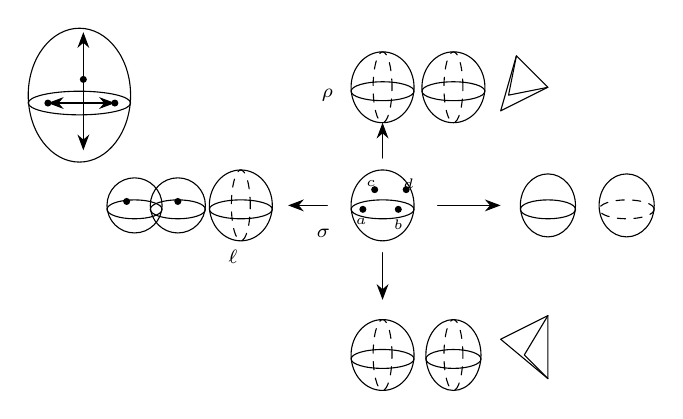
\begin{tikzpicture}[x=1mm,y=1mm,line cap=round,line join=round,font=\scriptsize]
\draw (13.5,-12) ellipse[x radius=6.5, y radius=8.5];
\draw (13.5,-13) ellipse[x radius=6.5, y radius=1.5];
\draw[-{Stealth[length=2mm]}] (14,-13) -- (14,-4);
\draw[-{Stealth[length=2mm]}] (14,-13) -- (14,-19);
\draw[-{Stealth[length=2mm]}] (14,-13) -- (9.5,-13);
\draw[-{Stealth[length=2mm]}] (14,-13) -- (18,-13);
\node[pt] at (9.5,-13) {};
\node[pt] at (18,-13) {};
\node[pt] at (14,-10) {};
\draw (52,-26) ellipse[x radius=4, y radius=4.5];
\draw (52,-26.5) ellipse[x radius=4, y radius=1.2];
\node[pt] at (49.5,-26.5) {};
\node[pt] at (54,-26.5) {};
\node[pt] at (51,-24) {};
\node[pt] at (55,-24) {};
\node[inner sep=1pt] at (49.3,-28) {\tiny $a$};
\node[inner sep=1pt] at (54,-28.5) {\tiny $b$};
\node[inner sep=1pt] at (50.5,-23.2) {\tiny $c$};
\node[inner sep=1pt] at (55.3,-23.2) {\tiny $d$};
\draw[-{Stealth[length=2mm]}] (52,-20) -- (52,-15.5);
\node[inner sep=1pt] at (45,-12) {\scriptsize $\rho$};
\draw[-{Stealth[length=2mm]}] (45,-26) -- (40,-26);
\node[inner sep=1pt] at (44.5,-29.5) {\scriptsize $\sigma$};
\draw[-{Stealth[length=2mm]}] (59,-26) -- (67,-26);
\draw[-{Stealth[length=2mm]}] (52,-32) -- (52,-38);
\draw (52,-11) ellipse[x radius=4, y radius=4.5];
\draw (52,-11.5) ellipse[x radius=4, y radius=1.2];
\draw[dashed] (52,-11) ellipse[x radius=1.2, y radius=4.5];
\draw (61,-11) ellipse[x radius=4, y radius=4.5];
\draw (61,-11.5) ellipse[x radius=4, y radius=1.2];
\draw[dashed] (61,-11) ellipse[x radius=1.2, y radius=4.5];
\draw (69,-7) -- (67,-14) -- (73,-11) -- cycle;
\draw (69,-7) -- (68,-12) -- (73,-11);
\draw (34,-26) ellipse[x radius=4, y radius=4.5];
\draw (34,-26.5) ellipse[x radius=4, y radius=1.2];
\draw[dashed] (34,-26) ellipse[x radius=1.2, y radius=4.5];
\draw (20.5,-26) ellipse[x radius=3.5, y radius=3.5];
\draw (20.5,-26.5) ellipse[x radius=3.5, y radius=1.2];
\node[pt] at (19.5,-25.5) {};
\draw (26,-26) ellipse[x radius=3.5, y radius=3.5];
\draw (26,-26.5) ellipse[x radius=3.5, y radius=1.2];
\node[pt] at (26,-25.5) {};
\node[inner sep=1pt] at (33,-32.5) {\scriptsize $\ell$};
\draw (73,-26) ellipse[x radius=3.5, y radius=4];
\draw (73,-26.5) ellipse[x radius=3.5, y radius=1.2];
\draw (83,-26) ellipse[x radius=3.5, y radius=4];
\draw[dashed] (83,-26.5) ellipse[x radius=3.5, y radius=1.2];
\draw (52,-45) ellipse[x radius=4, y radius=4.5];
\draw (52,-45.5) ellipse[x radius=4, y radius=1.2];
\draw[dashed] (52,-45) ellipse[x radius=1.2, y radius=4.5];
\draw (61,-45) ellipse[x radius=3.5, y radius=4.5];
\draw (61,-45.5) ellipse[x radius=3.5, y radius=1.2];
\draw[dashed] (61,-45) ellipse[x radius=1.2, y radius=4.5];
\draw (73,-40) -- (67,-43) -- (73,-48) -- cycle;
\draw (73,-40) -- (70,-45) -- (73,-48);
\end{tikzpicture}
\end{document}
